%!TEX root = ../DevaramaniS-[RnD-MT]Report.tex

\chapter{Experimental Evaluation and Results}

The following chapter presents the \textit{proof of concept} and evaluation of the proposed extension to \textit{Popov-Vereshchagin solver} . All the experiments are conducted in a simulation environment. The obtained results are analyzed based on the physical behavior of the system. 


\section{Experimental Setup}
This section describes the overall experimental setup followed to show the proposed extension to the solver for a mobile base. All the experiments discussed in the following sections are tested in a simulation environment. There are mainly three cases discussed in experimental setup. By varying the inputs to the solver, the obtained simulation results are analyzed based on the possible physical behavior of the system. 

The inputs to the solver are, robot model, inertia data, $q$, $\dot{q}$, $\tau$, $\ddot{X}_0$, $F^{ext}$, $A_N$ and $b_N$. The robot model is the created kinematic tree structure of the MPO-700 robot base, in the previous chapter. Some of the input parameters that are kept constant throughout the experiment, they are,

\begin{itemize}
	\item \textit{Input joint angles (q), velocities ($\dot{q}$) and accelerations ($\ddot{q}$)} = 0 for all joints
	\item \textit{Linear constraint matrix ($A_N$):} This defines the directions of the acceleration constraints on the end-effectors (wheels). In our case, the wheels are constrained along \textit{linear-y} (sliding constraint), \textit{linear-z} (no acceleration perpendicular to the ground) and \textit{angular-x} (wheel should not ``roll'' about x-axis). The $A_N$ matrix described for all the wheels is given by, 
	\begin{equation}
		A_N = \begin{pmatrix}
		 0 & 0 & 1 \\
		 0 & 0 & 0 \\
		 0 & 0 & 0 \\
		 0 & 0 & 0 \\
		 1 & 0 & 0 \\
		 0 & 1 & 0 \\
		\end{pmatrix}
	\end{equation} 
	\item \textit{Beta vector ($b_N$):} This defines the acceleration energy vector corresponding to directions of applied constraints. Since the wheels are constrained to not to have acceleration along linear-y, linear-z and angular-z, the $b_N$ vector for each wheels is given by,
	\begin{equation}
		b_N = \begin{pmatrix}
		0 \\
		0 \\
		0
		\end{pmatrix}
	\end{equation}
\end{itemize}

The two other input parameters are external force and feed-forward torques. In the following experiment scenarios, these two parameters are varied and the results are analyzed.  
The solver outputs are $\ddot{q}$, $\tau_{control}$ and $\ddot{X}$. 
\begin{itemize}
	\item \textit{Joint accelerations ($\ddot{q}$):} Represents the resultant accelerations at every joints. For simplified notations, the orientation joints are denoted by ``o'' and drive joints are denoted by ``d''. In the table below, the order of all the joint acceleration are - [o1, d1, o2, d2, o3, d3, o4, d4].
	\item \textit{Base acceleration:} Describes the Cartesian acceleration of the mobile base.
	\item \textit{Control torques ($\tau_{control}$):} Represents the resultant control torques of every joints (o1, d1, o2, d2, o3, d3, o4, d4). 
\end{itemize} 

Below table displays the simulation results. In the following sections each of the cases and its results are analyzed.

\begin{table}[h!]
	
	\renewcommand{\arraystretch}{2.2}
	\resizebox{\textwidth}{3.5cm}{%
		\begin{tabular}{| l | l | l | l | l |}
			\hline
			\multicolumn{2}{| M{7.5cm}|}{\textbf{Inputs}}    & \multicolumn{3}{M{15cm}|}{\textbf{Outputs}} \\ \hline
			
			\textbf{External force ($F_{ext}$)} & \textbf{Feedforward Torques($\tau$)} & \textbf{Joint accelerations ($\Ddot{q}$)} & \textbf{Base acceleration} & \textbf{Control torques ($\tau_{control}$)} \\ \hline
			
			\begin{tabular}[c]{@{}l@{}}$\tau_z = 10$ \\ $[0, 0, 0, 0,  0, 10]$ \end{tabular}   &  $[0, 0, 0, 0, 0, 0, 0, 0]$ &  \begin{tabular}[c]{@{}l@{}} $[-0.651743,   -1.36504, -3.97664,  -1.36552,$ \\ $-3.97664, -1.36552, -0.651743, -1.36504]$\end{tabular}   & \begin{tabular}[c]{@{}l@{}} $\dot{\omega}_z = 1.4962 $ \\  $\dot{v}_x = -0.0368095$ \end{tabular} & 	\begin{tabular}[c]{@{}l@{}} $[0.303226, -0, -0.126057, -0,$ \\$ -0.126057, -0, 0.303226, 0]$ \end{tabular} \\ \hline
			
			\begin{tabular}[c]{@{}l@{}}$f_x = 50$ \\ $[50, 0, 0, 0,  0, 0]$ \end{tabular}   &  $[0, 0, 0, 0, 0, 0, 0, 0]$ &  \begin{tabular}[c]{@{}l@{}} $[3.49264, 0.168407, 3.90164    0.168467,$ \\ $3.90164, 0.168467, 3.49264, 0.168407]$\end{tabular}   & \begin{tabular}[c]{@{}l@{}} $\dot{\omega}_z = -0.184047 $ \\  $\dot{v}_x = 0.158089$ \end{tabular} & 	\begin{tabular}[c]{@{}l@{}} $[0.243069, -0, 0.238214, -0 ,$ \\ $0.238214, -0, 0.243069, -0]$ \end{tabular} \\ \hline
			
			$F_{ext} = [0, 0, 0, 0,  0, 0]$  &  \begin{tabular}[c]{@{}l@{}} $\tau_{d_1} = 1.0$ \\ $\tau_{d_2} = 1.0$ \\ $\tau_{d_3} = 1.0$ \\ $\tau_{d_4} = 1.0$  \end{tabular} &  \begin{tabular}[c]{@{}l@{}} $[ 0.329141, 34.0727, 0.549795, 34.0727,$ \\  $0.757357, 34.1083, 0.12158, 34.1082]$\end{tabular}   & \begin{tabular}[c]{@{}l@{}}  $\dot{v}_x = 0.0111047$ \\ $\dot{v}_y = 0.00467013$ \\ $\dot{\omega}_z = -0.192697$ \end{tabular} & 	\begin{tabular}[c]{@{}l@{}} $[0.0695287, -0, -0.0665266, -0,$ \\ $-0.0539123, -0, 0.0463929, -0]$ \end{tabular} \\ \hline
		\end{tabular}
	}\renewcommand{\arraystretch}{3}
	\caption{Experimental analysis}
\label{tab:experiment}
	
\end{table}

\newpage

\section{Experiment 1:}

The first experiment corresponds to the first row in table \ref{tab:experiment}. As mentioned above, the quantities, $q$, $\dot{q}$, $\ddot{q}$, $A_N$ and $b_N$ are kept constant. In the first experiment, only the external torque ($\tau_z$) of 10 units is applied to the base and joint torques is zero. On applying torque of 10N on a rigid-body system, it is expected to produce certain angular acceleration at base. The relation between torque and angular acceleration is given by,

\begin{equation}
	\tau = I_{z} \dot{\omega}_z
\end{equation}

Here, $I_z$ represents the rotational inertia of the body. For the base, $I_z = 3.69$ as obtained from the URDF model. From the above relation, the angular acceleration will be $\dot{\omega}_z = 2.71$ rad/$s^2$. This result is 

{\color{red}Justifications on joint acceleration and control torques}

\begin{figure}[h!]
	\begin{center}
		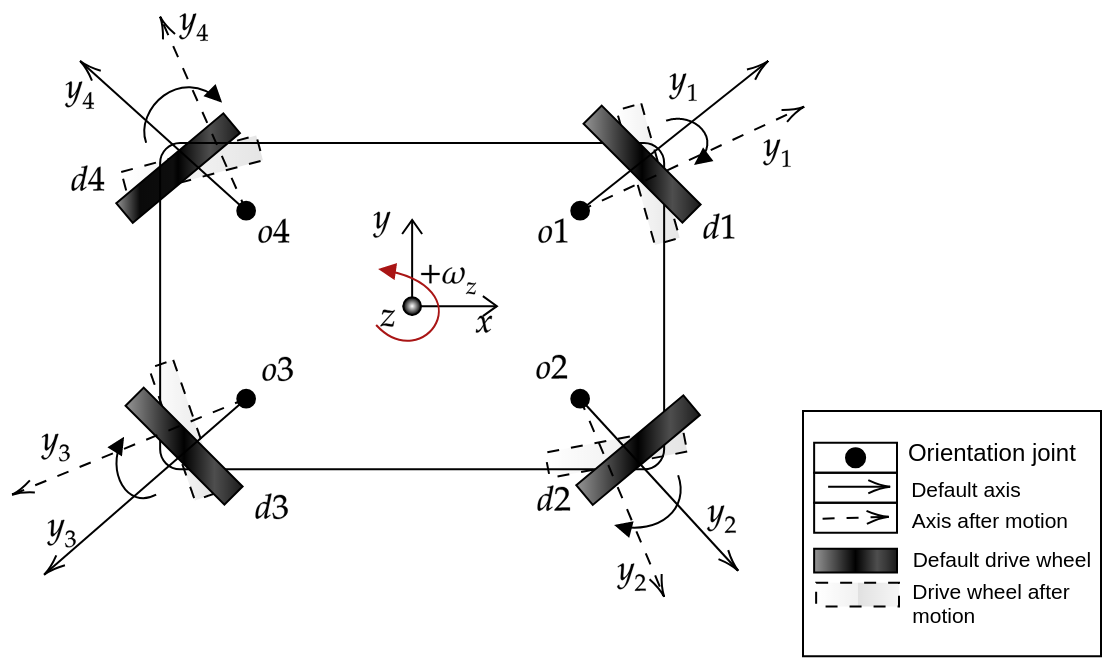
\includegraphics[scale=0.35]{images/exp1_1.png}
	\end{center}
	\caption{Experiment 1}
\end{figure}

\newpage
\section{Experiment 2}
In this experiment, an external force in linear \textit{x} direction is applied on the robot base, i.e., $f_x = 50$ and joint torques is 0. This external force causes the castor wheels to align in the direction of applied force and results in a non-zero linear acceleration at base ($\dot{v}_x = 0.158$). The well-known relation between force and acceleration according to Newton's second law of motion~\cite{newton1833philosophiae} is,

\begin{equation}\label{eq:f=ma}
	f_x = m \dot{v}_x
\end{equation}

Here, $m = 180$, mass of base (as given in the URDF model of MPO-700). By substituting the known variables in the equation \ref{eq:f=ma}, yields linear acceleration $\dot{v}_x = 0.277$ SI units. The error ($\delta$) between the calculated and the obtained acceleration value, $\delta = 0.119$. (Justification on error.......)

Additionally, the applied force produces angular acceleration about z. The relation between linear force and angular acceleration is,

...............


\section{Experiment 3}
In this experiment, no external force is given, the joint torques are applied to drive wheels that are equal to 1.0 SI units. In a physical system, the joint torques applied to the wheels result in acceleration of the system. The results show that the base has acceleration along linear-x, linear-y and angular-z. 
